\chapter*{Introduction}
\addcontentsline{toc}{chapter}{Introduction}
\chaptermark{Introduction}
\label{sec:background}
A fundamental grasp of the data that is produced by sequencing biological organisms is essential to comprehend the research outlined in this manuscript. If already familiar with DNA sequences, how they are obtained and how they differ between species or individuals, you may proceed to section~\ref{sec:background:pangenomics} \emph{From reads to \kmers}.
\section*{DNA, genome variation and sequencing data}
\label{sec:dna}
DNA (Deoxyribonucleic Acid) is a complex molecule with a double helix structure that carries the genetic information of an organism. Although its discovery was the result of work by many scientists over nearly 90 years, the currently accepted model was first correctly described by James Watson and Francis Crick in 1953 at Cambridge, UK.\\
The information DNA carries provides instructions for an organism to develop, survive in the external world, and reproduce. These instructions are encoded as a sequence of monomers called nucleotides. Each nucleotide is composed of a sugar, a phosphate group, and one of four nucleobases: cytosine, guanine, adenine, and thymine. The nucleotides are commonly referred to using the first letter of their nucleobases: A, C, G, and T. In RNA molecules, thymine is replaced by uracil.\\
The nucleotides are linked together in a sugar-phosphate backbone. Hydrogen bonds between complementary nucleotides form the molecule's double-stranded structure, with A pairing with T and C pairing with G bases. This pairing is crucial for DNA replication and protein synthesis. Figure~\ref{fig:DNA} shows the structure of the DNA molecule and the nucleotides, with the initial drawing by Francis Crick in 1953.
\begin{figure}[h!]
	\centering
	\begin{subfigure}[b]{0.95\textwidth}
		\centering
		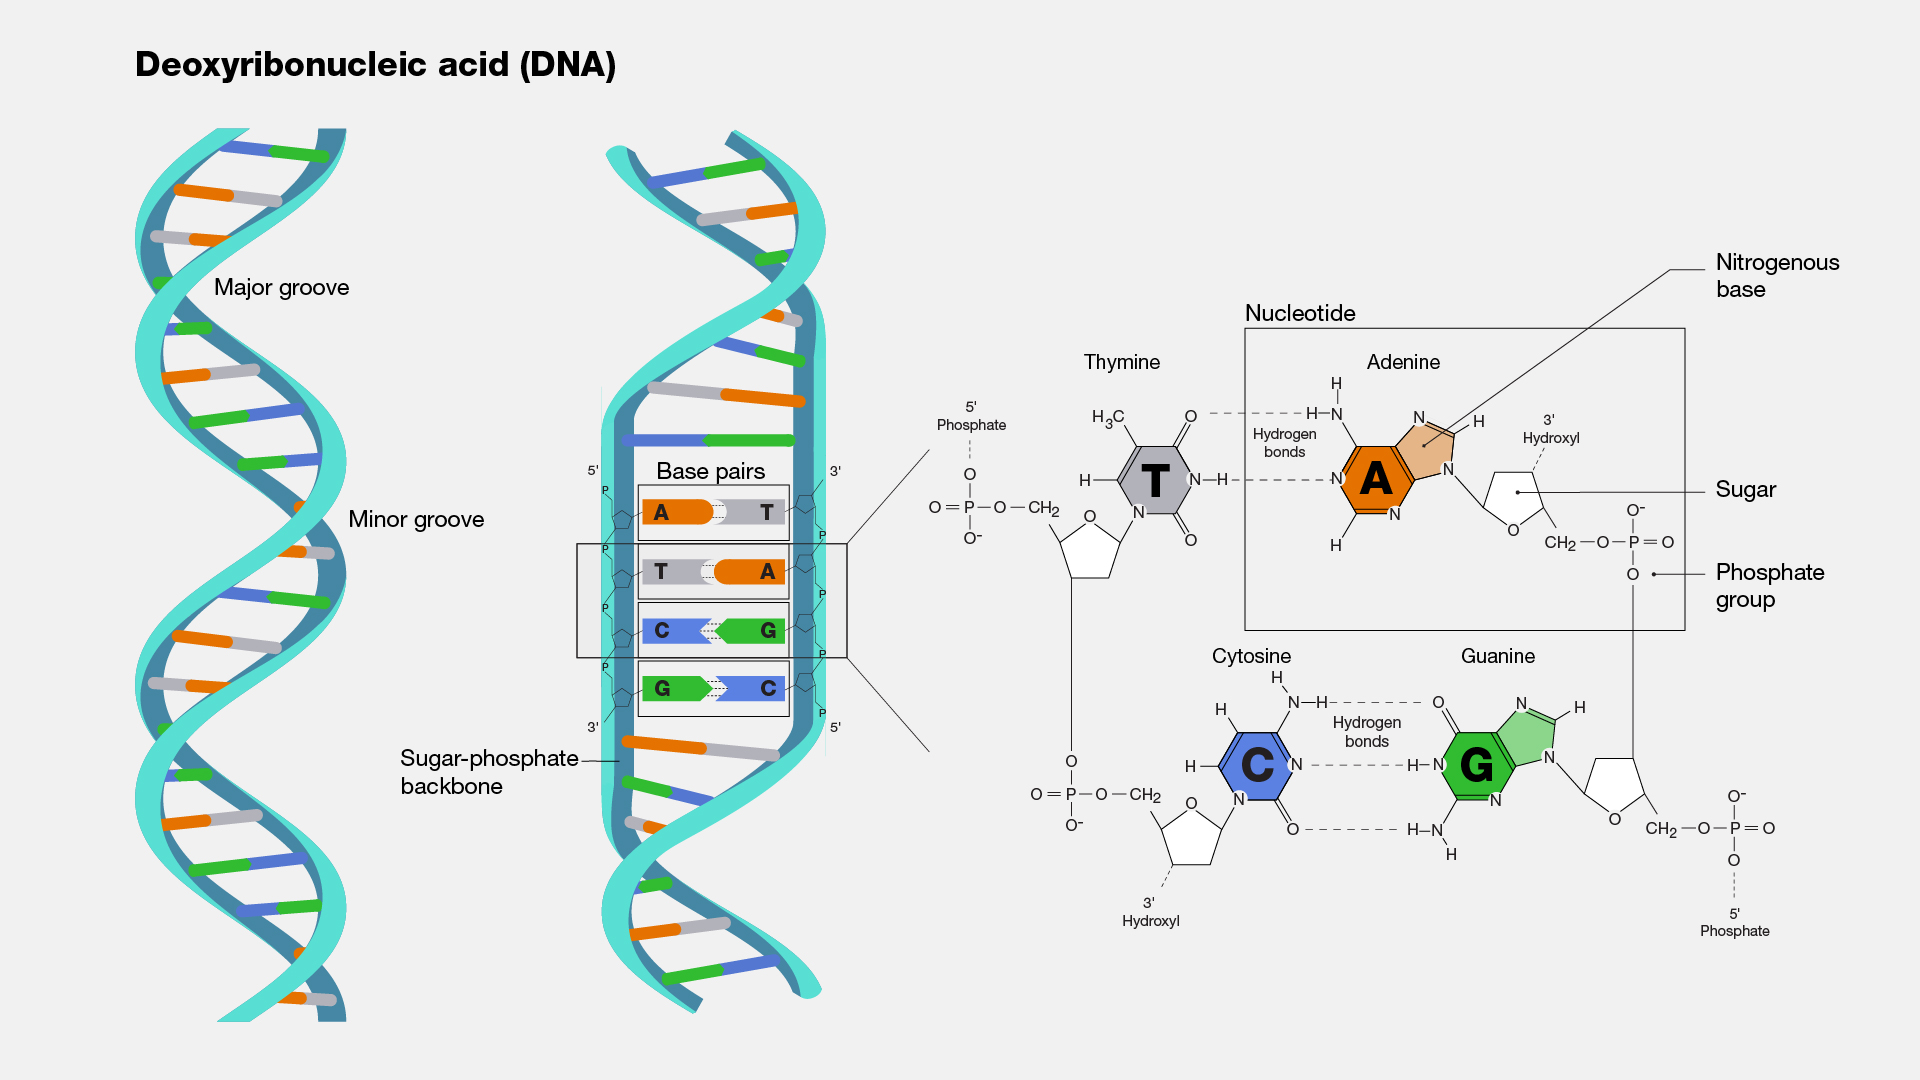
\includegraphics[width=0.95\textwidth]{figures/background/DNA_2024a.jpg}
		\caption[The DNA molecule]{The DNA molecule and the structure of the nucleotides, the basic piece of information of the DNA. Figure from NIH glossary~\cite{nih_dna}.} 
	\end{subfigure}%
	\\
	\begin{subfigure}[b]{0.75\textwidth}
		\centering
		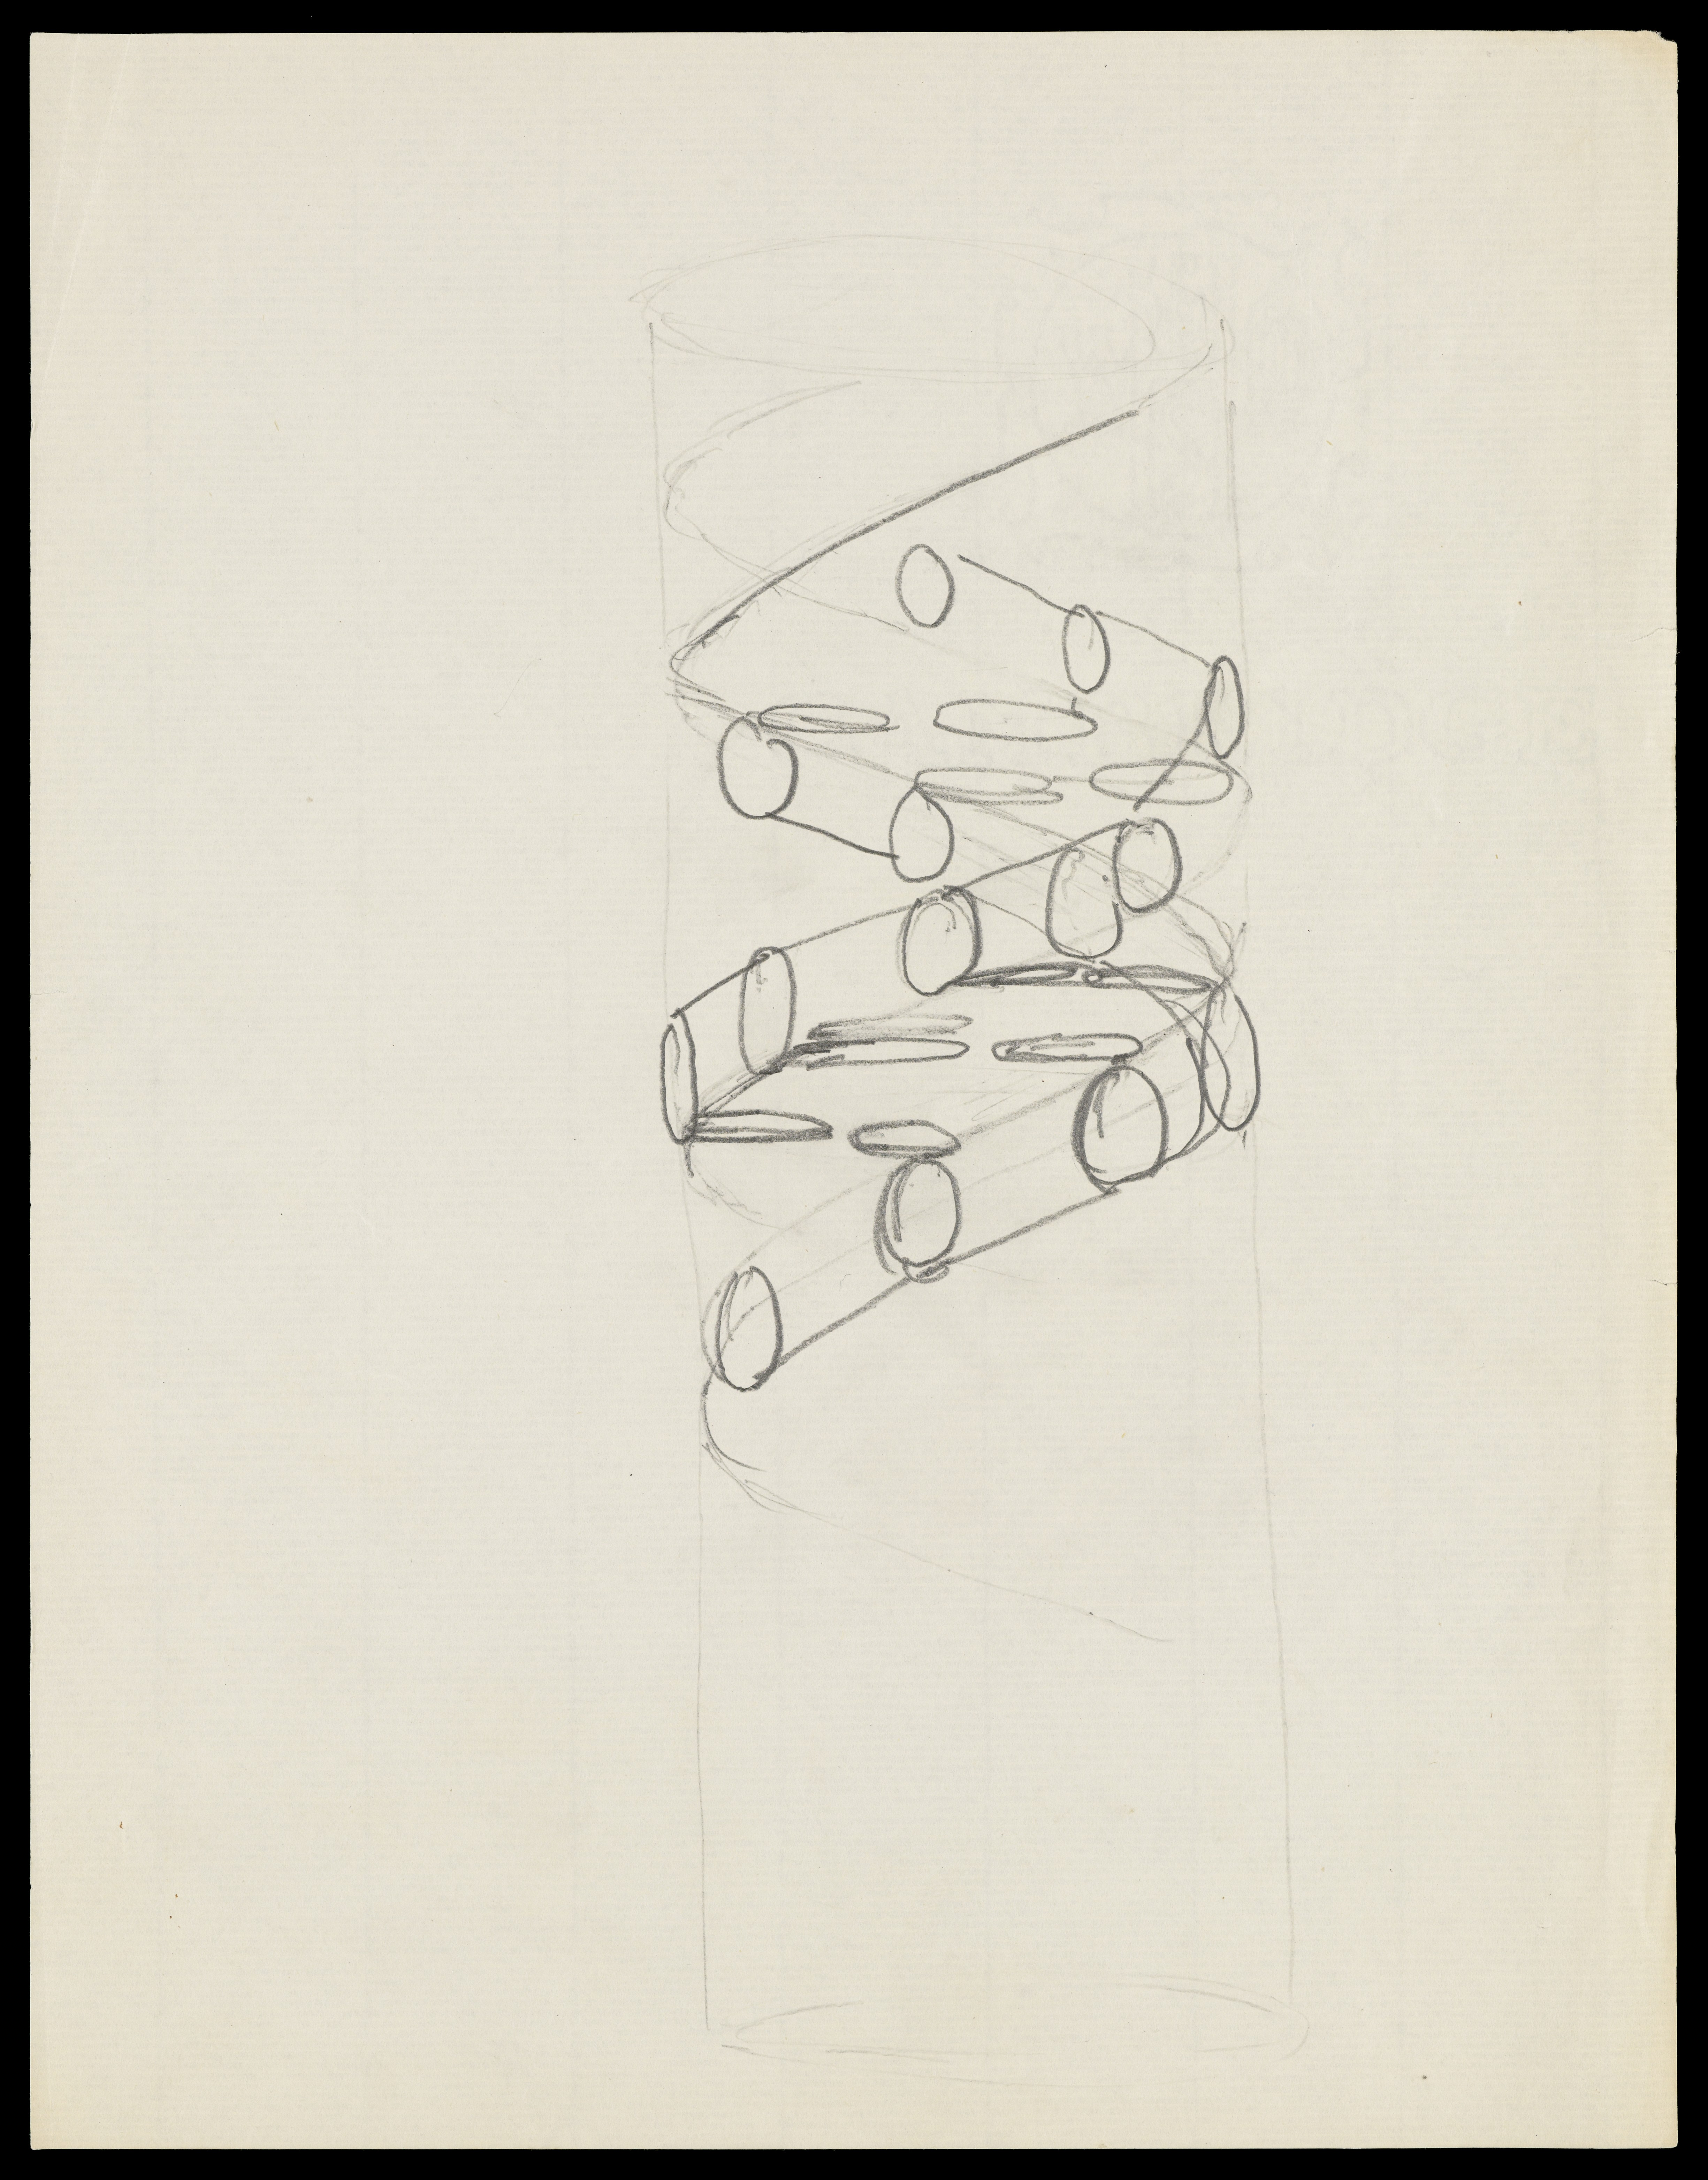
\includegraphics[width=0.5\textwidth]{figures/background/DNA_sketch.jpg}
		\caption[The DNA sketch by Crick]{The DNA molecule model draw by Francis Crick in 1953.} 
	\end{subfigure}%
\caption{The DNA molecule.}
\label{fig:DNA}
\end{figure}

To fit inside the cell nucleus, DNA is organized in very tight structures. First is coiled around proteins called histones to from a compact structure called chromatin that form loops and is kept in place by other molecules to structure a chromosome. Chromosomes are inherited by the offspring through sexual or asexual reproduction. Humans are diploids, i.e. contain 2 copies of the same chromosome, that receive one copy from the mother (the egg) and one from the father (the sperm). Both the egg and the sperm (the gametes) contain 1 copy of the chromosomes. While mammals are often diploids, other organism can be haploid (one single copy of the chromosome) or polyploid, i.e. have more than 2 copies. For example, the sugar cane plant, the world's most harvested crop by tonnage, can have more than 8 copies of a chromosome, up to 12~\cite{sugarcane}.
In humans, each nucleus of non-reproductive cells contains 23 chromosome pairs. 22 are the autosomes, i.e. the chromosomes we all have and that are not associated with sex, while the last pair is the sex one that contains or 2 copies of chromosome X for women or 1 X and 1 Y for men. The final part of the chromosome is called telomere while the central one is called centromere and both are regions known to contain a lot of repetitive regions that are very difficult to reconstruct from sequencing. \\ Finally, there is also the mitochondrial genome, that is not in the nucleus, has circular structure and is mostly inherited maternally.

\subsection*{DNA sequencing}
In many biological disciplines, studying an organism's genetic information contained in its DNA is crucial. Over the years, researchers have developed various methods and techniques to extract this information from the cell nucleus and to represent it in a useful way. These processes typically involve three main steps. Here I describe them, with many simplifications, to give a brief overview:
\begin{itemize}[leftmargin=1.8cm]
	\item[\textbf{Library preparation}] The first step requires hours long, nontrivial biological manipulation of samples to extract DNA from cell nucleus and purify it without causing damage. This process isolates the genetic material from other cellular components, like RNA and proteins. The DNA molecule are fragmented into pieces of different length followed by $5\prime$ and $3\prime$ adapter ligation. Some technologies require PCR amplification of fragments, while others don't.
	\item[\textbf{Sequencing}] Next, specialized machines detect the sequence of nucleotides that compose the extracted DNA pieces. These techniques, called sequencing, use various, most of the time proprietary, technologies to determine the precise order of nucleotides (A, C, G, and T) in a DNA molecule. The raw data output of these machines are sequences of characters that are referred to as sequencing reads or simply reads.
	\item[\textbf{Analysis}] In this step usually quality control (QC) is performed to remove adapters and too short or low quality reads. Usually the first step after QC is to assemble the sequences together or to provide them as input to a workflow specific for the required application.
\end{itemize}
The landscape of DNA sequencing has evolved significantly since its inception. In 1977, Frederick Sanger and his colleagues introduced the first widely adopted sequencing method, known as chain termination sequencing or Sanger sequencing\cite{sanger_sequencing}. This technique allowed to read the sequence of nucleotides in a DNA molecule for the first time in a reliable and reproducible manner. This was the technique that led to the first sequencing of the mitochondrial DNA and the first ,almost, complete human genome in 2001~\cite{mitochondrialDNA,first_human_genome}.
While Sanger sequencing has revolutionized genetic research, it has largely been replaced by more advanced technologies. These newer methods fall into two main categories: Next Generation Sequencing (NGS) and Third Generation Sequencing. These technologies provide significant improvements in terms of speed, cost-effectiveness and data output compared to Sanger sequencing. \\
\subsubsection*{Next Generation Sequencing} (NGS) derives its name by launching a so-called next generation by revolutionizing sequencing with massive parallelization. This technology has continuously improved since 2005 to yield up to 8 Terabases per single sequencing run, taking it maximum 2 days and dropping the price of, for example, a single individual sequenced per almost 100 dollars~\cite{100dollars}. The advancement consists mainly in running many reactions and analysis in parallel to produce millions to billions of reads of a length that varies between 150 and 300 bases. For this reason they take the name of short reads. While a big advantage of this sequencing method is the low error rates, with at least 80\% of the bases with less than 1 error in 1000 (i.e. 99.9\% accuracy). This technology is mostly dominated by a California biotechnology company called Illumina \\
The sequence length is the main drawback of this method, as it makes it difficult or impossible to resolve complex large-size DNA variations, where the read won't align to any part of a reference genome to be used to infer from which part of a chromosome it comes from. The same problem arise for repetitive regions,like centromeres, telomeres or small segmental duplications, that have a length greater than the sequence length, where it is not possible to asses the length or the nature of the repetition.
This problem has been partially addressed by the introduction of pair-end sequences, a technology that is now integrated in all Next Generation machines, that sequences both ends of a single DNA fragment and then associate the two reads that come from it, in order to provide more long-range information. Although this method is still not enough to solve complex structural variations or repetitive regions, it is very useful to track some of the reads that would be instead be unused and finds relevant applications in assembly or metagenomics. In fact, I used this property of paired-end reads in one method I developed before the PhD to improve the estimation of different species inside metagenomic samples sequenced with Next Generation Sequencing~\cite{metaprob2}. \\
\subsubsection*{Third Generation Sequencing} (TGS) is the newest technology that uses alternative approaches to NGS, to solve the issues that it currently face due to the short length of the sequences. The main difference relies on the fact that while NGS uses PCR to amplify the small fragments in which DNA is broken into prior to sequencing, these new technologies directly sequence the DNA molecule. Here I will describe the two most important technologies, provided by the two companies that lead this market: a California biotech company called Pacific Biosciences, usually called PacBio, and a Uk based one, called Oxford Nanopore Technologies, or ONT.\\
PacBio offers "HiFi sequecing" that produces reads long up to 25 thousands bases in length with accuracy comparable to NGS ones. This is achieved by first creating a circularized DNA from high-quality double stranded DNA and then using a DNA polymerase enzyme to read multiple times the same molecule to produce a final consensus sequence with accuracy of around 99.9\%. These are long and accurate reads that enable ultra-fast assembly of human genomes~\cite{mdbg} at a cost around \$1000 per sequencing reagents kit. \\
Oxford Nanopore machines instead provide ultra-long sequences, that are on average longer than the PacBio HiFi ones and can reach up to the megabase scale (i.e. ~100 times longer). The sequencing is done by passing a single-strand DNA molecule trough a tiny nanopore. Each pore is associated to an electrode and a sensor that measure the current that is passing through the pore. As the DNA goes through the pore, the current changes and, thanks to a basecalling algorithm, it is possible to detect the nucleotides by the change in the current. This process is done in parallel across ~800-1500 pores.\\
It is finally important to stress that these two technologies allow the detection of all kind of variations, i.e. small variations as well as large ones and also solve large repetitive regions as they span acorss thousands of bases. Moreover, both these methods allow the direct detection of DNA methylation. This is a chemical mechanism on top of the DNA molecule that regulates gene expression  by recruiting proteins involved in gene repression or by inhibiting the binding of transcription factor(s) to DNA~\cite{methylation}. \\
Figure~\ref{fig:sequencing_technologies} shows basic schematics of how these two technologies work.\\ 
\begin{figure}[h!]
	\centering
	\begin{subfigure}[b]{0.95\textwidth}
		\centering
		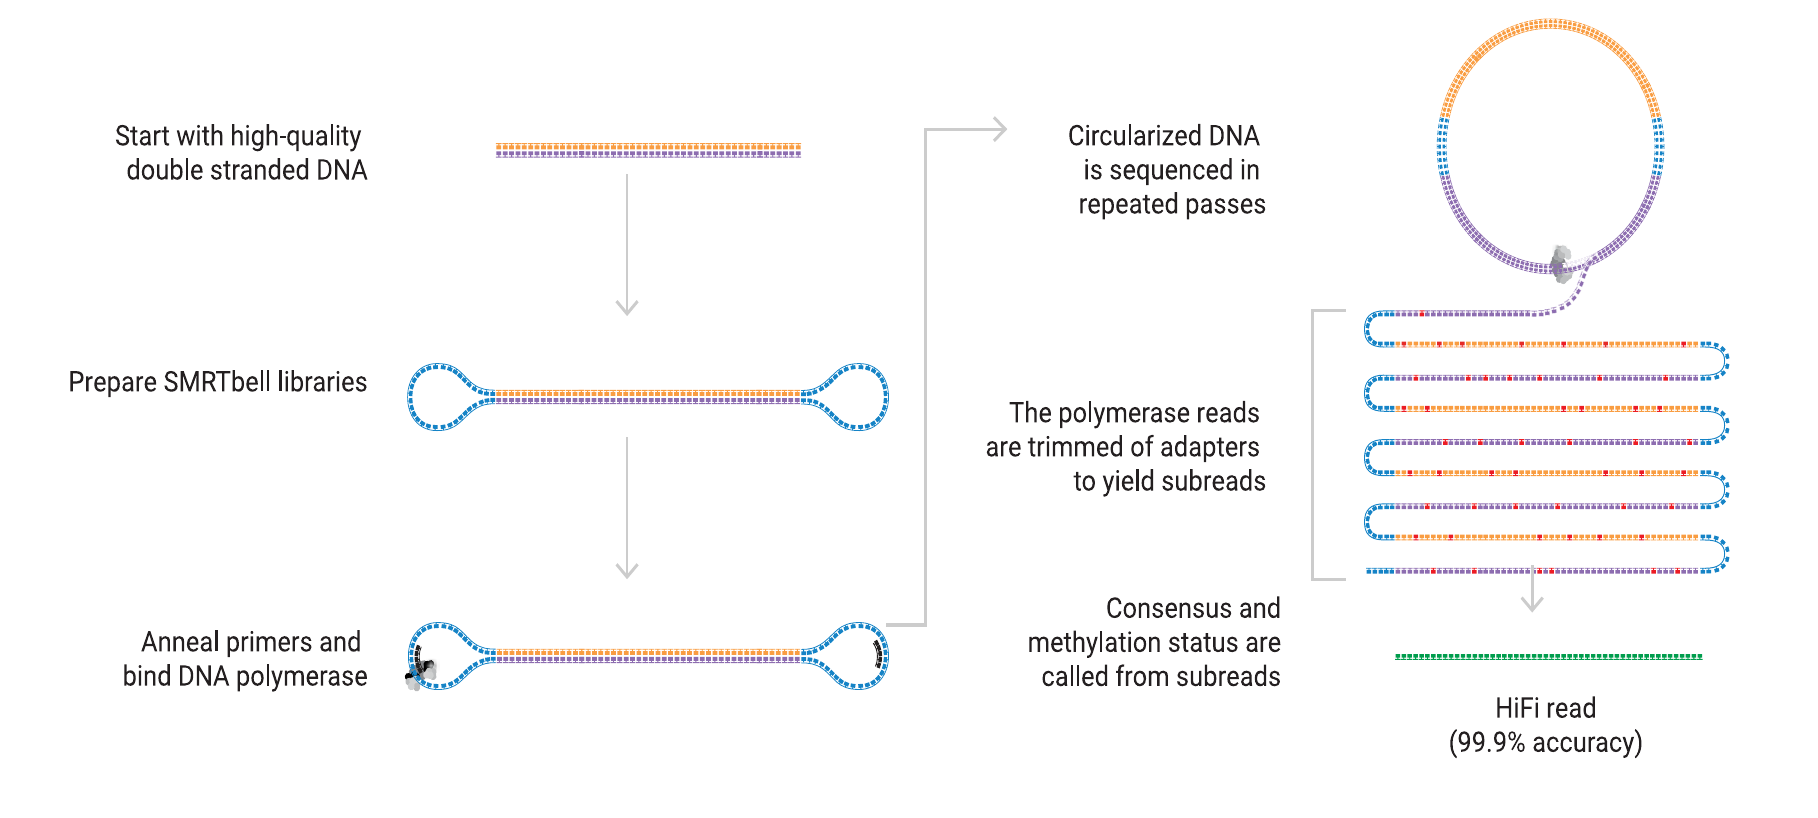
\includegraphics[width=0.95\textwidth]{figures/background/hifi_pacbio.png}
		\caption{Pacific Biosciences Hi-Fi reads generations scheme. Image from PacBio website.} 
	\end{subfigure}%
	\\
	\begin{subfigure}[b]{0.95\textwidth}
		\centering
		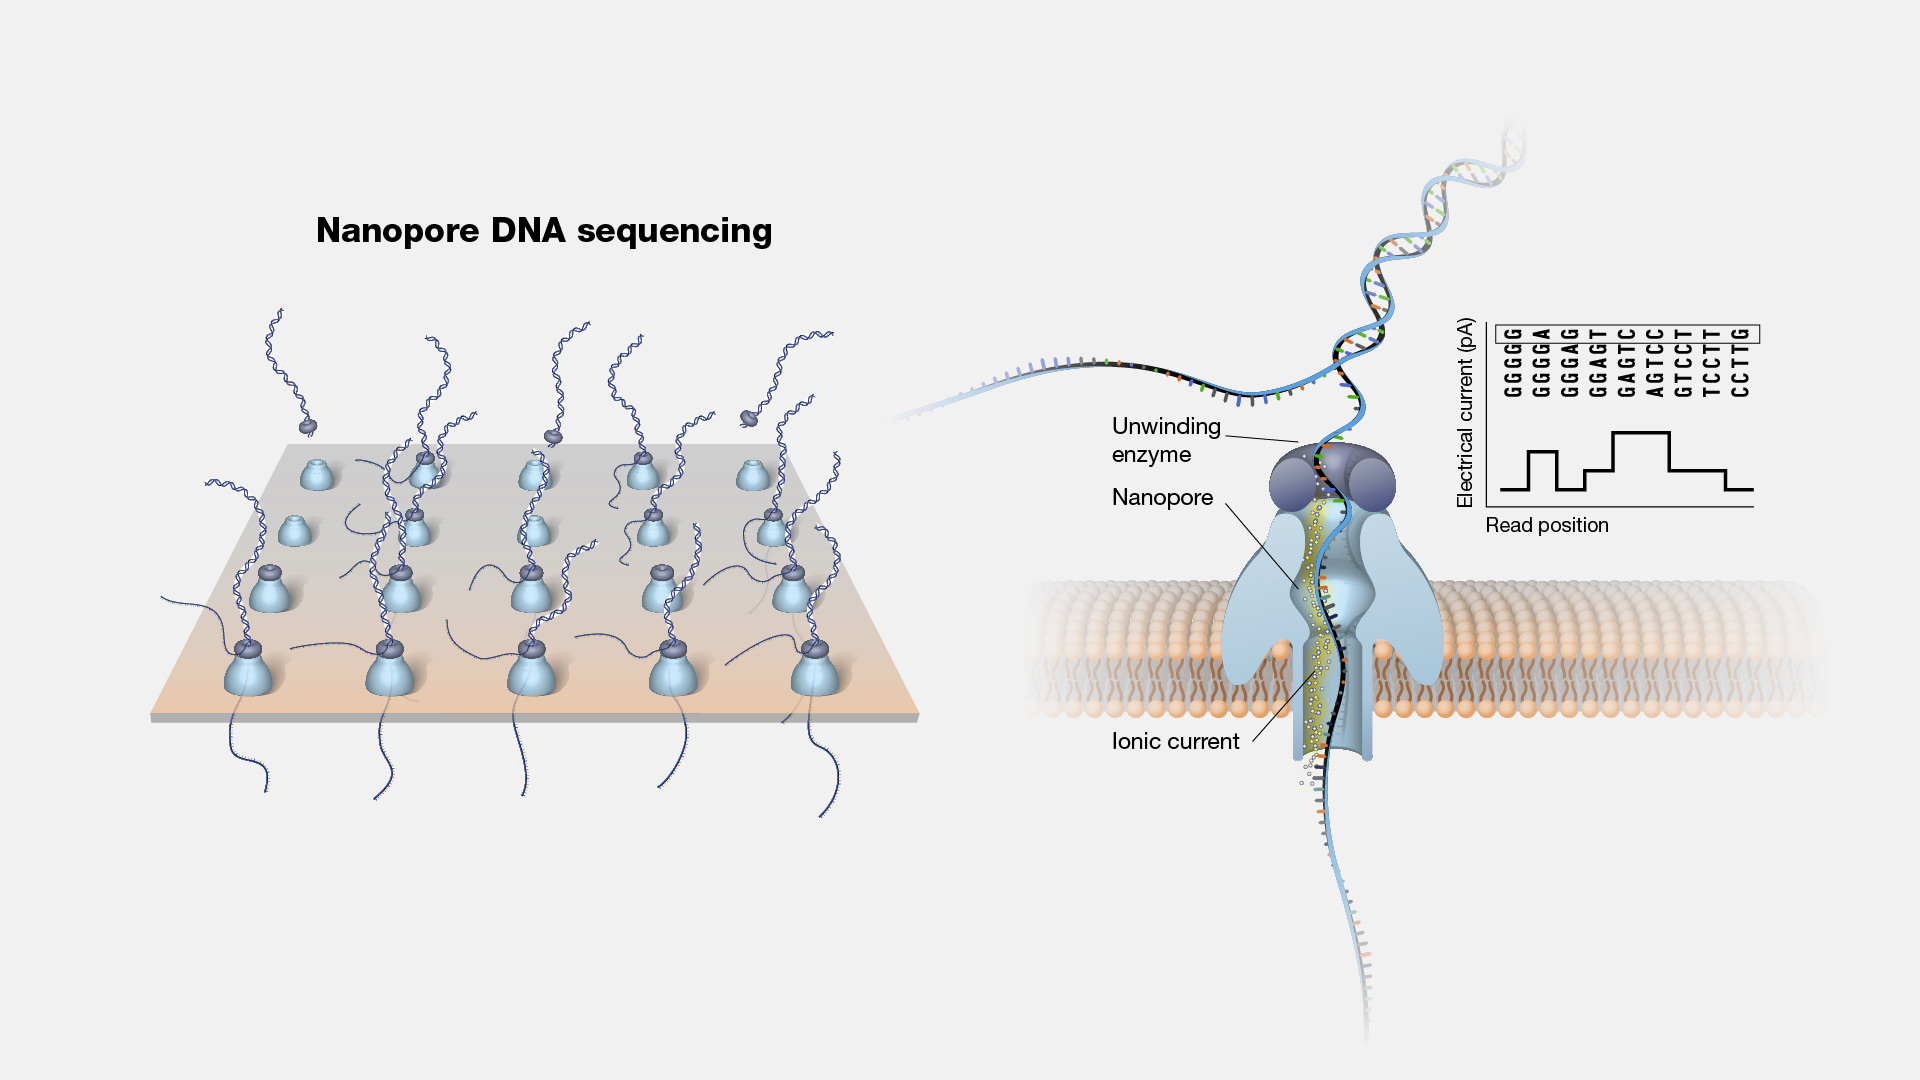
\includegraphics[width=0.95\textwidth]{figures/background/nanopore_sequencing.jpg}
		\caption{An array of pores sequences multiple molecules in parallel. A dsDNA molecule is split by the helicase enzyme and then a ssDNA sequence slowly gets through the pore for sequencing. Changes in the ionic current is used by a machine learning algorithm to infer the nucleotides of the sequence.} 
	\end{subfigure}%
	\caption{Third generation sequencing technologies.}
	\label{fig:sequencing_technologies}
\end{figure}

\section*{From reads to \kmers}
The sequences produced by any of the aforementioned technologies are considered as text strings, i.e. successions of characters, like the phrases of this manuscript, in which each character correspond to a nucleotide. These sequences can therefore being stored in plain text formats, like FASTQ, that preserve basecalling quality information or in others, like FASTA, that retains only the actual sequence. In order to use less space and take advantage of redundancy in the sequencing data, these files are often compressed, using one of the many tools publicly available like \texttt{gzip} or \texttt{zstd}, by Facebook. \\
As pair-end short-reads have different features than ultra-long reads or Hi-Fi long reads, most of the tools focus on providing applications for just one single type. In cases like assembling a genome from the reads or calling the variant of the sequenced genome compared to one of reference, however, the information from different sources can be combined to provide superior results. In order to generate high-quality genome assemblies, for example, many consortia, like the Human Pangenome Reference Consortium, use Hi-Fi long reads as bases for assembly plus ultra-long reads as scaffolds to chain together the assemblies into sequences that span from telomere to telomere of a chromosome.\\
In the work presented in this manuscript, most of the tools will ingest as input or raw sequences (both NGS or TGS) or high-quality, near telomere-to-telomere assemblies. Some of the tools that I have have used and all of the ones I have developed or co-developed transform the input sequences or assemblies into \kmers to produce the desired output. \\
\begin{description}
	\item[DNA alphabet] The DNA alphabet $\sum$ is composed by the 4 characters that compose the first letter of the nucleobases: A,C, G and T: $ \sum = {A, C, G, T}$, 
	\item[sequence] a biological sequence from $\sum$ is defined as $ S =\in \sum^{l}, with \lvert S \rvert = l $, with length $l$ that can be fixed, if originated from NGS, or variable, if originated from TGS.
	\item[\kmer] a \kmer of $S$ is defined as $ \kmer \in \sum^{k}, with \lvert \kmer \rvert = k  $ i.e. any valid substring of $S$ of length $k$. 
\end{description}
As shown in table~\ref{tab-kmers}, from any sequence $S$, it is possible to obtain its constituent \kmers. To efficiently extract all \kmers from a sequence, the best approach is to employ a sliding window technique. This is done by identifying the first \kmer at the start of the string and then iteratively shifting the window one position at a time, appending the newly encountered character to the right while removing the leftmost character.\\ The length $k$ of a \kmer is an arbitrary value, that is usually chosen depending on the kind of sequences used (cannot have $k$ > $n$), the characteristics of the data that is used (is it from a single organism, a collection of the same species, a collection of different organisms) and on the disk or memory space that is available for computation or storage (as in table~\ref{tab-kmers}, the longer the $k$, the more space is used by repetitive characters). A more detailed explanation of these considerations will be provided in section XXX[QF].\\
As it is possible to retrieve \kmers from a single read, it is trivial to extend this property to any set of reads, for example produced by a single sequencing run of a sample. This means that a set of \kmers is equivalent to the set of reads it is obtained from. In order to characterize this transformation as lossless, i.e. without any loss of information, an association from each \kmer to the read(s) it comes from would be needed. In most of the cases this is not useful and \kmers are obtained from reads without remembering from which reads do they come from. In other, specific, applications it might instead be needed to know in which reads there are certain \kmers. More considerations on this are going to be presented in section XXX[BackToSequences].\\
As presented in section~\ref{sec:dna} the DNA is double-stranded, with A bases are paired with T ones, while C bases are paired with G ones, also called complements. If a \kmer appears in a sequence, in the other strand of the molecule there would be what is called its reverse complement. This is the spelling of the \kmer from the end to the beginning, substituting each base with its complement. For example if in one strand there appear the sequence $ACGT$, on the other strand it would spell $TGCA$.\\
When enumerating \kmers from a sequence or when storing them, only "canonical" \kmers are kept: this means that for each \kmer produced from a sequence, its reverse-complement is computed and only the one that is considered smaller by a certain property is kept. For example, if the lexicographic order is used, the \kmer (with $k=4$) $ACGT$ is lexicographically smaller than $TGCA$ so when either of the two is seen, only the first is kept.\\
A classic operation that is done when enumerating \kmers from sequences is to keep track of how many times each canonical \kmer appears in the set of sequences. This is called \kmer counting and finds important applications in many genomic disciplines like metagenomics or transcriptomics.\\
\kmers are being used in lots of applications based on NGS short reads while they are less implied on methods for error-prone long reads because using \kmers on one side destroys the long range information provided by reads that span thousands of bases, on the other error-rates higher than NGS would produce too many erroneous \kmers that would be very difficult to correct if not with very deep sequencing, providing additional cost bottlenecks. With Hi-FI reads and improved quality of nanopore basecalling, it is possible to overcome the error limitation and use \kmers for long reads. One example that uses advanced concepts based on \kmers is the tool \mdbg that drastically improved assembly of Hi-Fi reads.\\ 
\begin{table}[h!]
\begin{center}

	\begin{tabular}{ c c c c c c c c c c c}
		\toprule
		Position & 1 & 2 & 3 & 4 & 5 & 6 & 7 & 8 & 9 & 10 \\
		\midrule
		Sequece $S$ & C & T & G & A & A & C & T &A & C & A\\
		\midrule 
		$3-mers$ & C & T & G  \\
		&   & T & G & A \\
		&   &  & G & A & A \\
		&   &  &  & A & A & C\\
		&   &  &  &  & A & C & T\\
		&   &  &  &  &  & C & T & A \\
		&   &  &  &  &  &  & T & A & C \\
		&   &  &  &  &  & & & A & C & A\\
		
		\hline
	\end{tabular}

	\vspace*{0.3 cm}

	\centering
	\begin{tabular}{ c c c c c c c c c c c}
	\toprule
	Position & 1 & 2 & 3 & 4 & 5 & 6 & 7 & 8 & 9 & 10 \\
	\midrule
	Sequece $S$ & C & T & G & A & A & C & T &A & C & A\\
	\midrule 
	$4-mers$ & C & T & G & A \\
	&   & T & G & A & A\\
	&   &  & G & A & A & C\\
	&   &  &  & A & A & C & T\\
	&   &  &  &  & A & C & T & A\\
	&   &  &  &  &  & C & T & A & C\\
	&   &  &  &  &  &  & T & A & C & A\\

	
	\bottomrule
\end{tabular}
	\caption{\kmers with $k=(3,4)$ being computed from the sequence $S = CTGAACTACA $. $l-k +1$ $k$-mers are generated for a total of $(l -k + 1) * k$ bases. While with $k=3$ the total bases are $ 8 * 3 = 24$, with $k=4$ they are instead $28$, as larger $k$ encodes more information redundancy.}
	\label{tab-kmers}
\end{center}
\end{table}


\begin{table}
\begin{center}
	\begin{tabular}{c | c}

		Sequence id & sequence \\
		\hline
		seq1 & ACATCA \\
		seq2 & CTTCAG \\
		seq3 & TACAGC \\
		seq4 & GCTTAC \\
		
	\end{tabular}
\newline
\vspace*{0.2 cm}
\newline

	\begin{tabular}{c | c | c | c  | c}

		Sequence id & seq1 & seq2 & seq3 & seq4\\
		\hline
		\kmers  & \underline{ACA} (TGT) & CTT (\underline{AAG}) & TAC (\underline{GTA}) & GCT (\underline{AGC}) \\
			    & CAT (\underline{ATG}) & TTC (\underline{GAA}) & \underline{ACA} (TGT) & CTT (\underline{AAG}) \\
				& \underline{ATC} (GAT) & \underline{TCA} (TGA) & \underline{CAG} (CTG) & TTA (\underline{TAA}) \\
				& TCA (\underline{TGA}) & \underline{CAG} (CTG) & \underline{AGC} (GCT) & TAC (\underline{GTA}) \\
	\end{tabular}
\newline
\vspace*{0.2 cm}
\newline

	\begin{tabular}{c | c}

		oredered caonical \kmer & count\\
		\hline
		AAG & 2 \\
		ACA & 2 \\
		AGC & 2 \\
		ATG & 1 \\
		ATC & 1 \\
		CAG & 2 \\
		GAA & 1 \\
		GTA & 2 \\
		TAA & 1 \\
		TCA & 2 \\
	\end{tabular}
\end{center}
	\caption{Example of canonical \kmers enumeration and count. Given a set of sequences, for each of them \kmers are computed in a stream. For each of them, on the fly, the reverse complement is computed. Then the ones that are considered canonicals are passed and counted.\\ In the table below, reverse complements are between parenthesis and the canonical between the two (by lexicographic order) is underlined.}
	\label{tab-lista-kmer}
\end{table}

\clearpage
\section*{Pangenomics, pangenomes and pangenome graphs}
\label{sec:background:pangenomics}
\subsection{Genetic diversity: focus on humans.}
%Genomic variations are the characteristics that produce differences between organism of a species or between species. 
The genetic diversity is the variability that exists between organisms at the genetic level, i.e. differences in the information enclosed in their DNA. It is the raw material for biological evolution as, without heritable genetic differences between us, we would not be able to biologically evolve. Here what I will present is valid for humans, as the large part of my work has been with human DNA sequences. Most genetic changes have no effect at all on the individuals carrying them but some can result in phenotypic differences.\\
\subsubsection{Causes and drivers of genetic diversity in humans}
There are two main mechanisms of genetic diversity: the arise of new mutations and the reshuffling of already present genetic material trough recombinations and duplications. Mutations are produced by physical or chemical damage, for example caused by UV radiation, prior cell division or by errors in the DNA replications during cell division. When this occurs in germinal cells they are transmitted to the offspring, while when happening in a somatic cell (not reproductive), the mutation is not transmitted but can instead be responsible for certain type of cancer. In humans, it is estimated that a newborn carries on average 70 point mutations (one nucleotide substitute with another), 15 from the mother and 55 from the father. The amount of mutations is proportional with the age of the person and, more than induced by replication, it is due to not corrected damage.\\
On top of the mutations, chunks of chromosomes from the mother and the father chromosomes are shuffled to produce new combinations. The effect of this random process produces the differences between siblings with the same biological parents. Recombination is heterogeneous in the DNA and depends on some motifs that promote higher recombination. Finally, recombination is also influenced by the age, mostly of the mother, as older mothers tend to produce offspring with more misplaced recombinations, also causing the well known trisomy 21.\\
Without diverging too deep into population genetics, it is also important to understand how new variations are conserved, lost or fixed (become prevalent) in a population. These outcomes are driven by two main factors: genetic drift and natural selection.\\
Genetic drift is a process, given by the randomness in the individuals that reproduce in a specific population. This can contribute to the loss or fixation of some variants just because of randomness and not because they provide an advantage to the individual. Specifically, in populations with small number of reproductive individuals, this can fixate detrimental variants, while in large populations, the large number of individuals buffers the event. \\
Natual selection, on the other hand, is a mechanism that explains human evolution: as genetic variations causes the gain or loss of specific phenotipic traits, these traits can confere positive or negative advantage compared to the rest of the individual in a population (fitness). This phenomenon can contribute selecting certain variations in a population by either contribute to the fixation or the loss of a variant. This mechanism explains our species adaptation to nutritional resources, climate and pathogenes: in 10 thousand years a mutation in a gene that conferred the ability to digest milk has almost got fixed in humans, selection on certain genes explains better adaptations to cold or high altitudes and selection in HbS or DARC alleles has helped humans adapt and survive malaria infections\cite{genome_diversity_quintana}. 
\subsubsection{Human Genomic variation: types of variants}
There are various types of genomic variants: from the shortest, the single-nucleotide variants (SNV) or Single Nucleotide Polimorphism (SNP) when it is present in at least 1\% of the population, is the difference of one nucleobase between two individuals. In a specific part of the genome one person can have instead of a cytosine (C) a thymine (T), like for the SNP located 14 thousands bases upstream of the lactase gene that enables the lactase persistence mentioned earlier\cite{lactase_persistance}.
A second group of small variants is made of insertions and deletions (called together \emph{indels}): these are events in which it is present or missing a group of less than 50 nucleotides. The number of nucleotides is an arbitrary threshold used to better separate them from other kind of variations. Specific types of indels are the tandem repeats that, as the names suggests, are insertions or deletions of small repeated sequences of DNA. These repetitions usually are one after the other with no other sequence in between~\cite{nih_variation}.\\
\begin{figure}[h!]
	\centering
	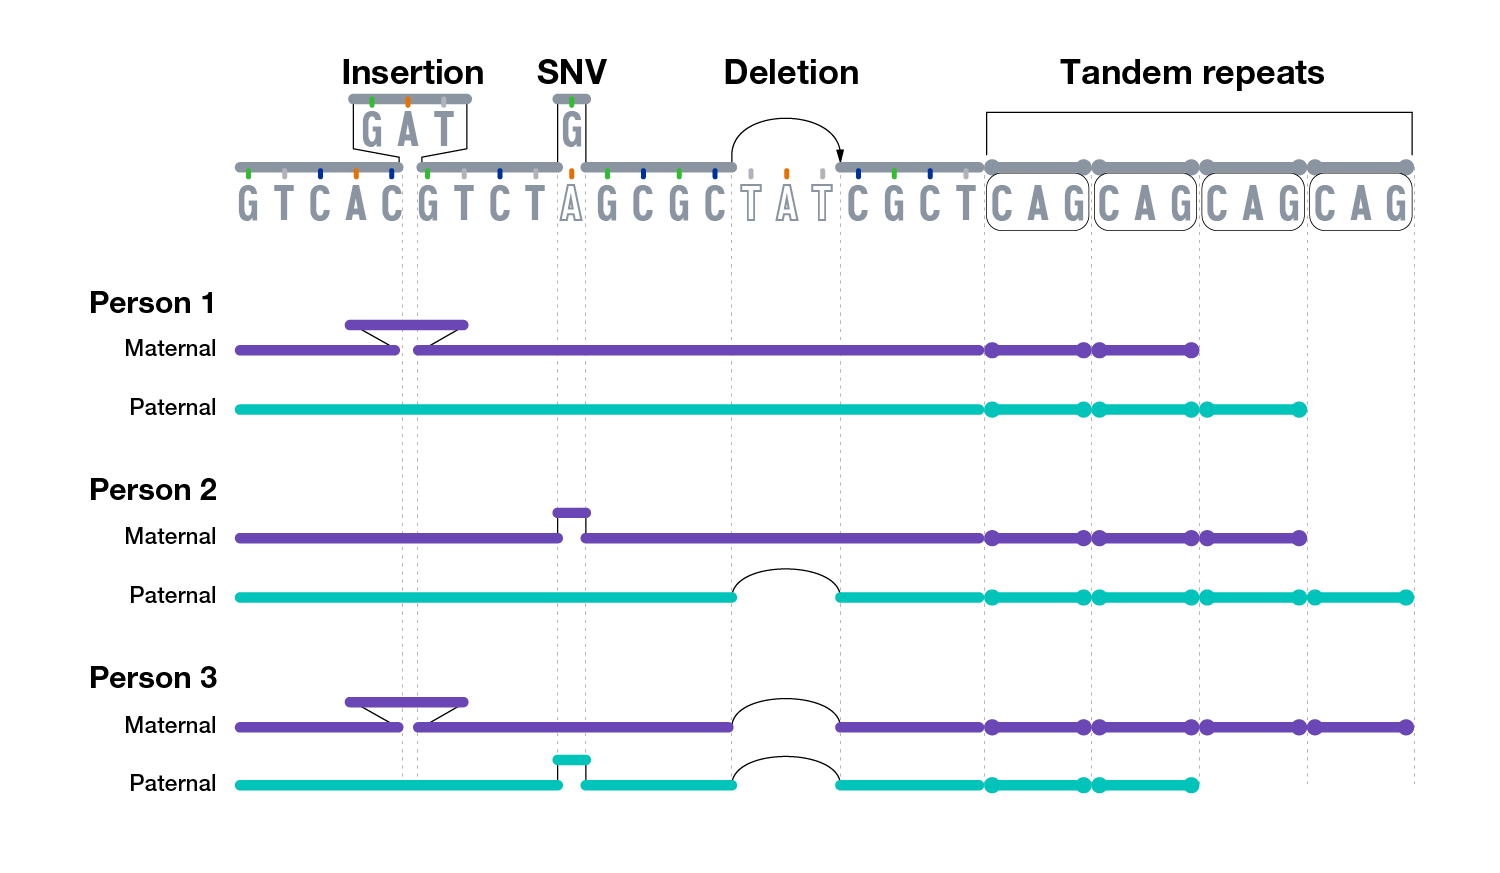
\includegraphics[width=.8\linewidth]{figures/background/small_variants.png}
	\caption[Small genomic variants.]{Graphic showing the types of small genomic variants~\cite{nih_variation}}
	\label{fig:small_variants}
\end{figure}
These groups of small variants, shown in figure\ref{} are the most described, studied and associated with diseases as they were the only one consistently detectable with NGS sequencing. For these reason, studies that tried to associate genomic variation with diseases commonly used only these kind of variants.\\
The other kind of variations are the ones that stretch at least 50 nucleobases and that can reach the dimension of large chunks of the chromosomes: they are called structural variations (SVs).
These can be indels or tandem repeats with the repeated section longer than 50 nucleotides, accounting for nearly half of all SVs, that take the name of Copy Number Variants (CNVs). Moreover, there are also inversions, in which a chunk of DNA is inverted compared to another and translocations in which pieces of two different chromosomes trade places~\cite{nih_variation}.\\
\begin{figure}[h!]
	\centering
	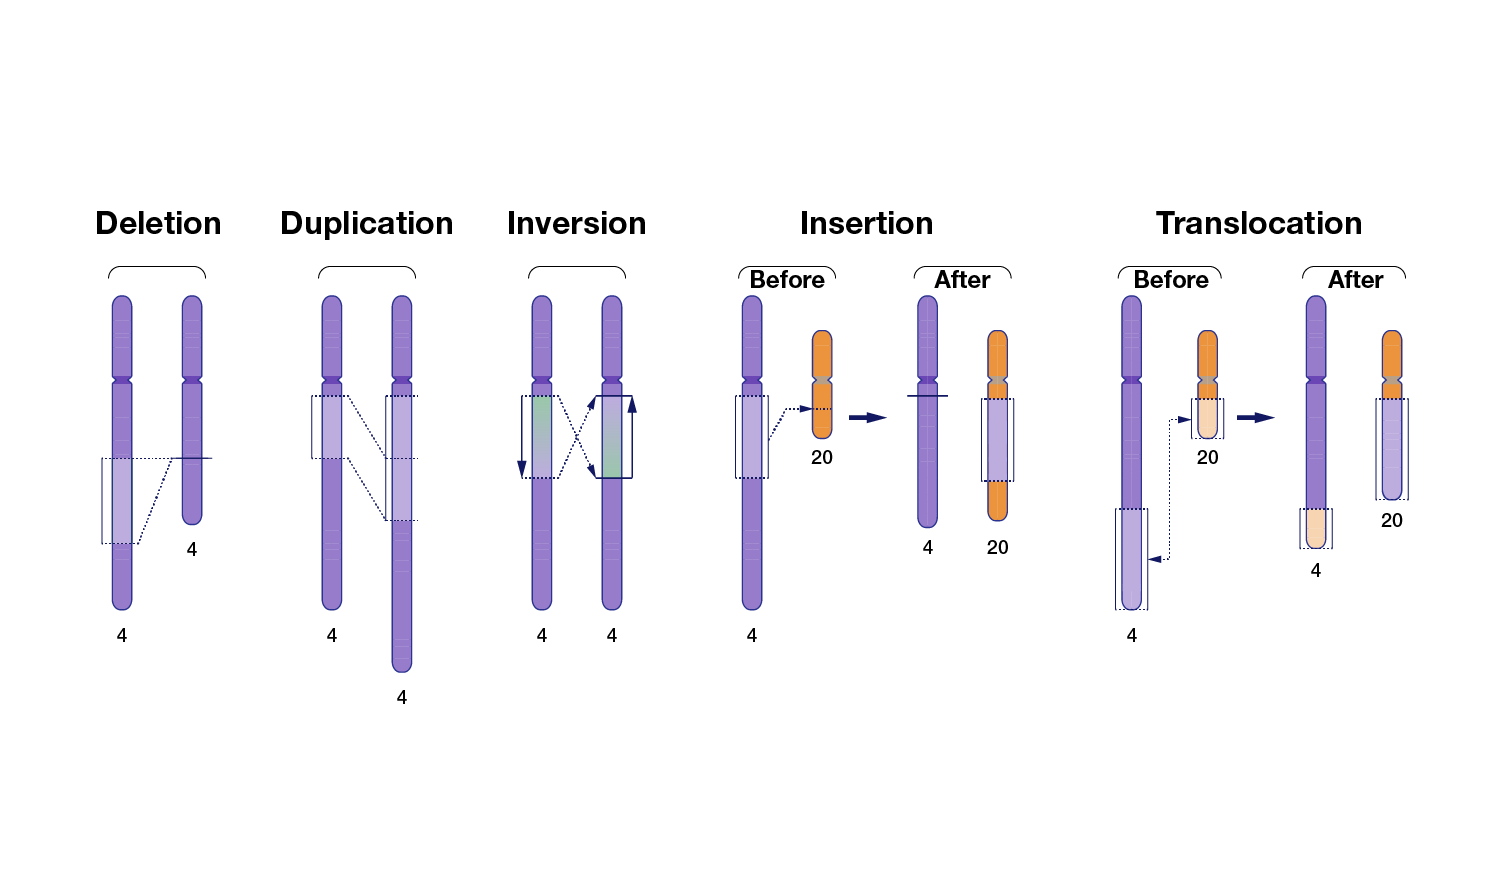
\includegraphics[width=.8\linewidth]{figures/background/large_variants.png}
	\caption[Large genomic variants.]{Graphic showing the types of large genomic variants~\cite{nih_variation}}
	\label{fig:large_variants}
\end{figure}
Finally, it is important to remember that these kind of variations can be on just one haplotype (copy of the chromosome) or on both: this distinguish between heterozygous and homozygous alleles.


\subsection*{The importance of studying genomic diversity in populations}
The Human genome contains more than 3 billions base pairs and contains probably more than 20 thousands protein coding genes, i.e. specific parts of the DNA that serve as blueprint for proteins. The rest is non-coding, i.e. is not a gene but can serve as regulatory element, like enhancers, promoters and silencers or as other conserved, functional element.\\
DNA differs between individuals of the same population (inter-individual) and between different populations of the same species (inter-population): figure~\ref{fig:pop_diff} shows these differences for four close primates. As discussed before, differences in DNA are given by having a different nucleotide at the same place (SNV), indels and large and complex variations, up to Megabases, that can produce different counts of copies or different ordering of a same region. \\
On average, each human carries around 10 thousands amino-acid altering mutations, 300-400 gene disruption events (like stop, splice and indels) affecting 200-300 genes and is heterozygous at 50-100 mutations associated with an inherited disorder~\cite{genome_diversity_quintana}. 
Finally, even when close species share a large portion of genetic material, structural changes that rearrange the same material in different order or invert it, contribute to meaningful changes. In figure~\ref{fig:chromosome_diff} it is shown how the chromosome 7 and 16 of some primates, even if very similar, differs in terms of organization. These large structure rearrangements are thus fundamental to understand the biology of organisms.
It is 
This is because the variation in DNA is produced by two main mechanisms: mutations and recombination. 

Moreover, genetic diversity is driven by two main factors: genetic drift and natural selection. Genomic duplication followed by adaptive mutation is considered one of the primary forces for evolution of new function
\begin{figure}[h!]
	\centering
	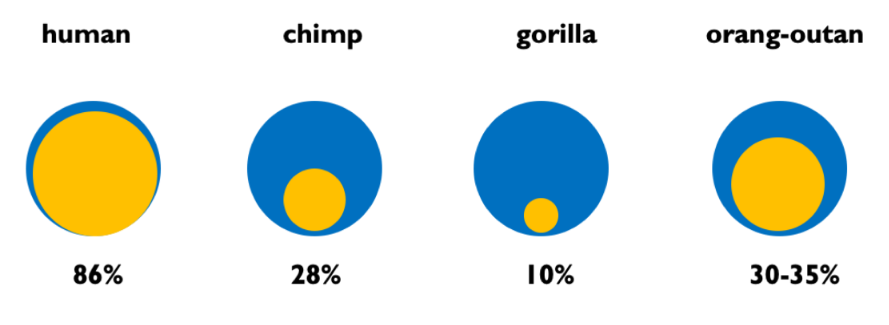
\includegraphics[width=.8\linewidth]{figures/background/pop_diff.png}
	\caption[Inter-individual and inter-population variation for 4 primate species.]{Share of inter-individual (yellow) and inter-population (blue) diversity for four different primates. While for humans the  majority of the diversity is within populations, for other primates it is between populations. This shows how Humans are more mixed than other primates. Percentage shows the inter-individual variation share~\cite{genome_diversity_quintana}.}
	\label{fig:pop_diff}
\end{figure}

\begin{figure}[h!]
	\centering
	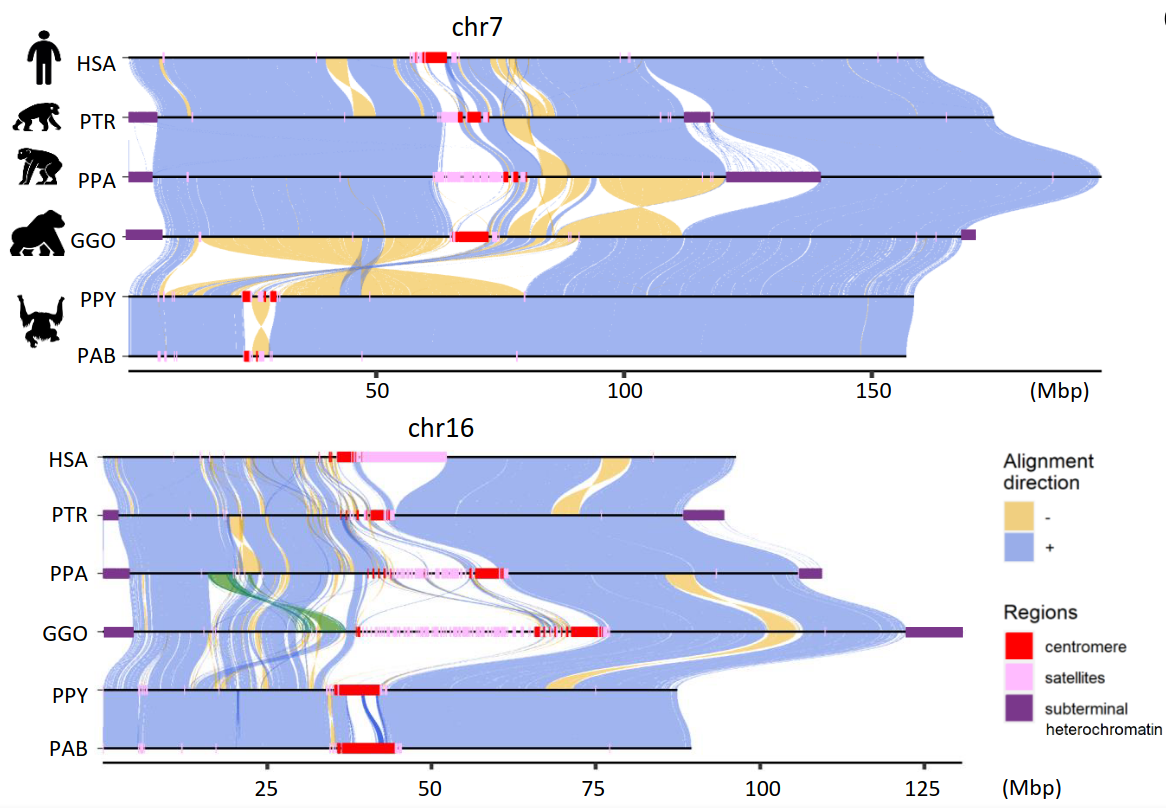
\includegraphics[width=.95\linewidth]{figures/background/genome_diff.png}
	\caption[Genomic difference in chromosome 7 and 16 of 5 primate species.]{A comparative ape alignment of human (HSA) chromosomes 7 and 16 with chimpanzee (PTR), bonobo (PPA), gorilla (GGO),Bornean and Sumatran orangutans (PPY and PAB). The image on the top shows most of the chromosome 7 is conserved except for large inversions happening between the species. The image below shows complex inversions in chromosome 16. Image taken from 'Complete sequencing of ape genomes'~\cite{ape_genomes}.}
	\label{fig:chromosome_diff}
\end{figure}

\begin{figure}[h!]\clearpage
	\centering
	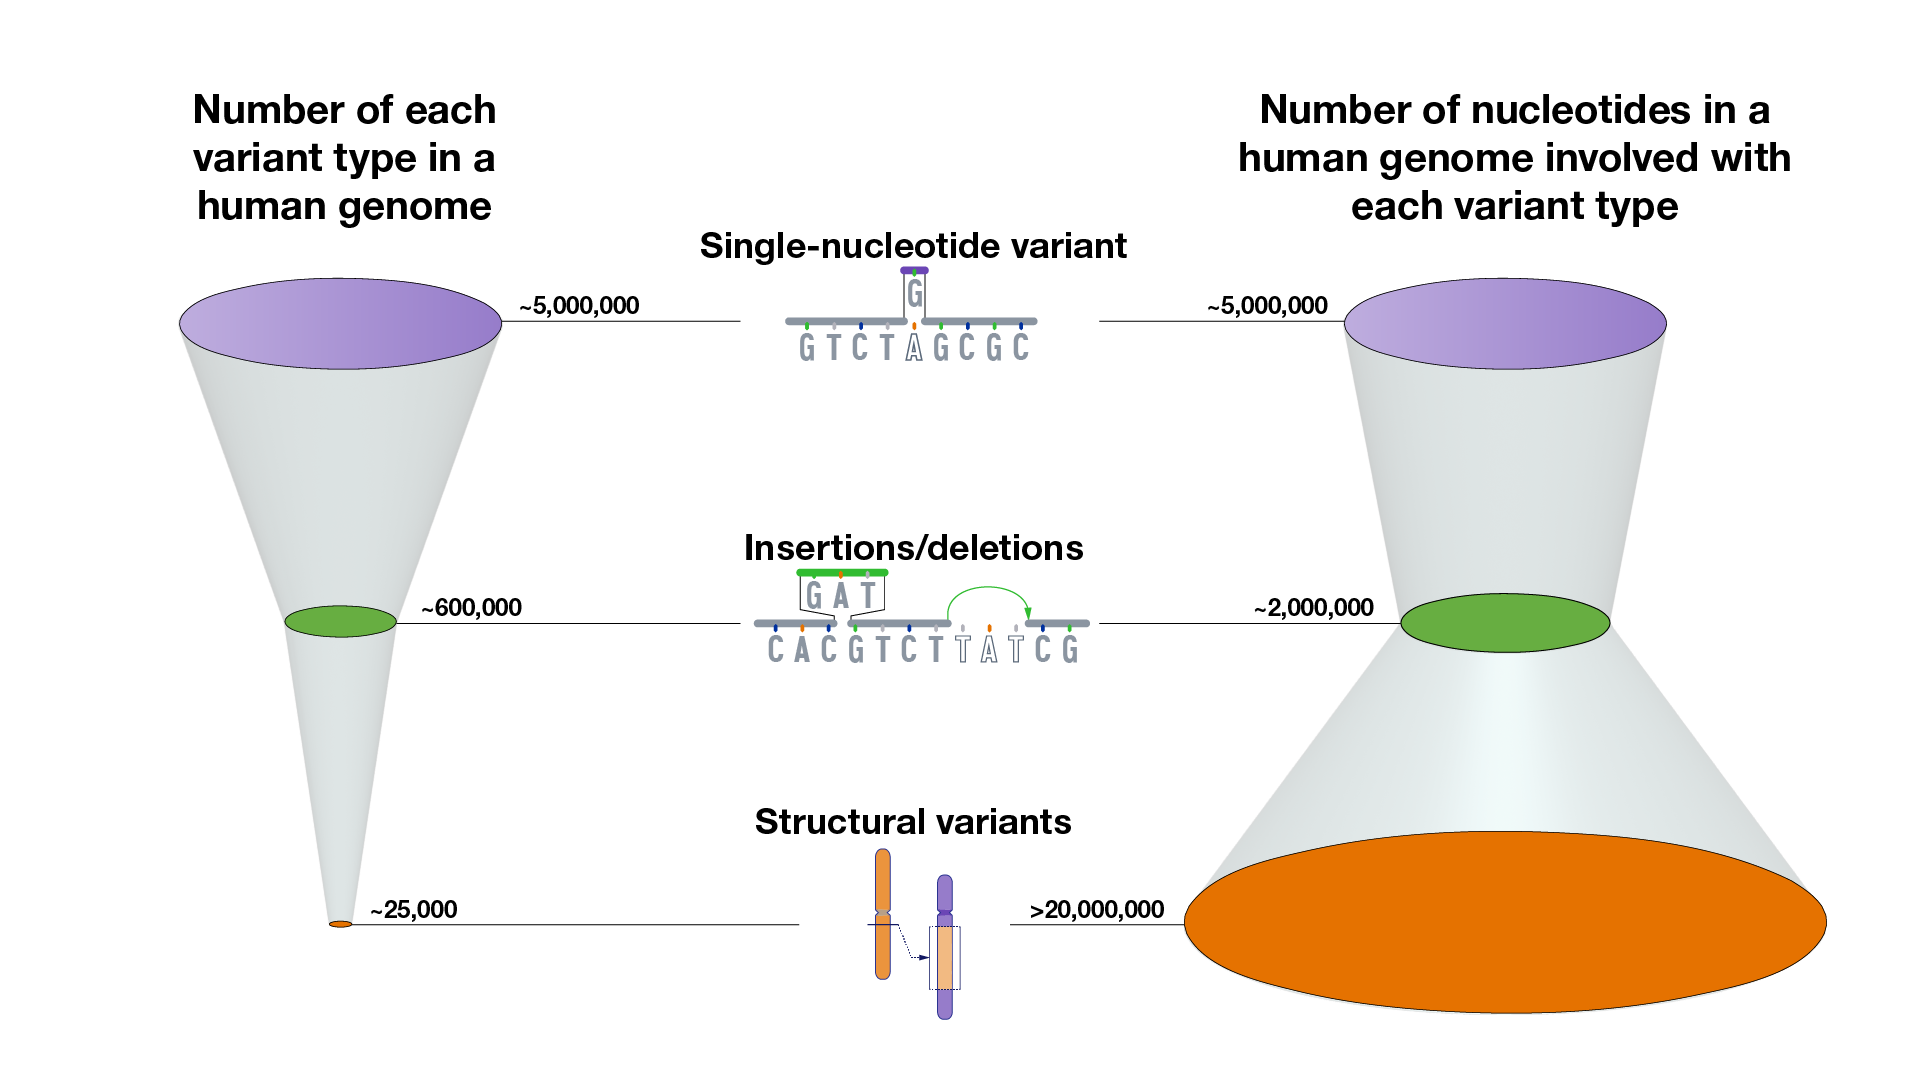
\includegraphics[width=.95\linewidth]{figures/background/genomic_spectrum.png}
	\caption[Spectrum of Human Genetic Variation.]{Spectrum of Human Genetic Variation. While SNPs are the most common variation event, their impact in the total amount of bases in a genome is ~4 times smaller than the one of Structural Variations, that are 200 times less frequent. This shows the great need to consider SVs in genomic analysis and not to stop at the SNP/indel level.\\}
	\label{fig:variation_spectrum}
\end{figure}

\subsection*{The premises for human pangenomics}
\textbf{A LINEAR REFERENCE FOR ALL GENOMIC ANALYSES}\\
Since the beginning of genomics, all analysis based on sequencing data depended upon the use of a single linear reference genome, i.e. the best assembled genome available for a species, to extract useful information from the DNA. We now know that this approach is suboptimal in a wide range of applications as a lot of genetic material of the species cannot be present in a single linear refererence: this is valid for eukariotes and even more for bacteria.  
\textbf{A SEQUENCING REVOLUTION}\\
Right now we are witnessing a real revolution in the sequencing. As the price is significantly lowering, also thanks to competition of new companies entering the market, new scientific discoveries and technological advances are leading to a remarkable increase of quality, in term of per-base error rate, and throughput. This means than right now we dispose of a rich wealth of high quality sequencing information to produce hundreds or thousands of new first grade assemblies.

\textbf{A QUALITY REVOLUTION}
This limitation at the beginning was not solvable due to the scarcity of high quality assembled genomes as the technologies of sequencing and computational tools were not mature enough. For example, the Human Genome Project took 13 years to produce its result~\cite{humangenomeproject} and the absence of long reads with decent error rate made it impossible to automatically resolve repetitive regions like telomers and centromeres~\cite{human-pangenomics-era}, producing a reference only $92\%$ complete~\cite{t2t}. This problem was only solved in 2022~\cite{t2t}. At the same time, many consortia are producing increasingly more genomes to a level comparable to the T2T consortium. For example, the HPRC, i.e. the Human Pangenome Reference Consortium released 47 new human genomes (92 haplotypes) in 2021 and has recently released other 153 genomes to a total of 400 haplotypes. The ability to produce such high quality data for human genomes is the main driver of the \\
Right now we are witnessing a real revolution in the sequencing. As the price is significantly lowering, also thanks to competition of new companies entering the market, new scientific discoveries and technological advances are leading to a remarkable increase of quality, in term of per-base error rate, and throughput. This means than right now we dispose of a rich wealth of high quality sequencing information to produce hundreds or thousands of new first grade assemblies.
This progress lead to a shift in paradigm with increasing effort from the scientific community to propose new methods to analyse one or multiple genomes: not anymore by comparing it against a single reference sequence but against a comprehensive representation of the species. \\
This novel way to overcome the limits of "linear genomic" and consider all the variation in a single species is called pangenomics. \\
Various efforts are being made on producing reference pangenomes of yeasts, bacterias, plants and animals, including humans. In order to do so, new tools to construct and then analyse and use such representations are being developed. 
It is important here to notice, as it will be stressed in the next sections and chapters, that construction is just the first step and that is very important to understand and work on which are the operations that can be succesfully performed by these representations. \\

\subsection*{Pangenomics}
\subsubsection*{Pangenomes}
\subsubsection*{Pangenome Graphs}

\section*{Graphs}

\subsection*{De Bruijn Graphs}
\subsubsection*{Colored and Compacted De Bruijn Graphs}
\subsection*{Variation Graphs}
\section*{Outline}
